\section{ISA}
Den Aufbau unserer Instruction Set Architecture haben wir bereits beim ersten Gruppentreffen begonnen und stark umstritten.
Im Verlauf des Projekts hat sich viel geändert, zum Teil motiviert durch Wünsche und Verbessungsideen unserer Mitglieder,
zum Teil begründet in Fehlern oder Problemen mit den Befehlsworten oder deren Bitcode-Layout, um die Interpretation des Binärcodes in der Hardware zu vereinfachen.
In der \autoref{AP:ISA} ist unsere endgültige Instruction Set Architecture zu sehen.

Von Beginn an war ein Reduced Instruction Set (RISC) mit drei Operanden-Befehlen geplant,
wobei wir uns an den Befehlssätzen der RISC-Prozessoren von ARM und MIPS orientiert haben.
Die Wortbreite beträgt 32-bit. Es gibt 15 General Purpose-Register, wovon zwei zum Speichern des Stack Pointers und der Rücksprungaddresse genutzt werden.
Das erste Register \texttt{\$0} ist immer null und kann auch zum Verwerfen eines Ergebnisses genutzt werden, in dem es als Zielregister angegeben wird.
Es gibt vier Statusflags -- Zero, Negative, Carry, Overflow.
Diese können von allen ALU-Befehlen gesetzt werden und für konditionierte Sprünge genutzt werden.
Mit dem \texttt{\$0}-Register und den Statusflags werden Vergleiche nun als Substraktionen modelliert:
Der Befehl \texttt{cmp \$1, \$2} wird übersetzt zu \texttt{subs \$0, \$1, \$2} --
also eine Substraktion, bei der die Statusflags abhängig vom Ergebnis gesetzt werden, und das Ergebnis in \texttt{\$0} gespeichert wird. \\
Alle ALU-Befehle können auch mit einem 16-Bit-Immediate als dritten Operanden genutzt werden.
In der finalen Version der ISA exisitiert kein Divisionsbefehl, da dieser zu Gunsten anderer Bitmasken-Befehle fallengelassen wurde.
Zudem gibt es keine Multiplikation, die ein 64-bittiges Ergebnis hat.

Für Speicherzugriffe gibt es zwei Load- und Store-Befehle zum Lesen und Speichern von 32-Bit-Wörtern --
die Speicheraddressen müssen dabei kein Vielfaches der Wortbreite sein.
Die Angabe der Speicheraddresse ist entweder absolut mittels eines Registers oder relativ zum Program Counter mit einem 24-Bit-Immediate.
Eine relativer Zugriff mit einem Register ist so nicht direkt möglich, aber der \texttt{adr}-Befehl kann für etwaige Addressberechnungen verwendet werden.
Zusätzlich gibt es die zwei Spezialbefehle \texttt{push} und \texttt{pop}, um die Stacknutzung zu beschleunigen.

Die Sprungbefehle sind ähnlich gehalten wie die Speicherbefehle und
können entweder absolut springen mit einem Registerwert oder PC-relativ mit einem 24-Bit-Immediate.
Zudem sind alle Sprungbefehle bedingt von den Statusflags.
Die Sprungbedingung ist eine Veroderung von einer beliebigen Teilmenge von Statusflags beziehungsweise eine Negation davon.
Hiermit können alle wichtigen Bedingungen dargestellt werden:
Ein positives Ergebnis lag zum Beispiel vor, wenn $\neg (\texttt{Negative} \lor \texttt{Zero})$ gilt.
Auch hier gibt es wieder einen Spezialbefehl zur Beschleunigung typischer Assemblerprogramme: den \texttt{call}-Befehl.
Diesen gibt es nur in der Ausführung PC-relativ mit Immediate.
Er speichert gleichzeitig den Wert \texttt{PC+4} im Rücksprungregister und
eignet sich damit hervorragend für Subroutinenaufrufe.

Schlussendlich haben sich in unserer ISA auch noch Befehle als nützlich erwiesen,
die eine spezielle Funktion direkt an der Hardwareschnittstellen des FPGAs abstrahieren.
Die ISA bietet uns die Möglichkeit, direkt auf Buttons und LEDs auf dem FPGA zuzugreifen.
Außerdem gibt es zwei Befehle zum Senden und Empfangen von Daten über die serielle Schnittstelle.
Wir sind diesem Weg gefolgt, da wir die Implementierung von Interrupts oder Maschinenregistern vermeiden wollten.
So ist die Lösung sehr einfach zu implementieren und zu nutzen, aber nicht sonderlich flexibel.

All diese Feinheiten der ISA haben sich mit der Zeit entwickelt.
Beginnend bei unserem Primärziel, ein FPGA zu einem kleinen Taschenrechner werden lassen, hatten wir eine entsprechend kleine ISA.
Sie umfasste lediglich den Befehlsatz für arithmetische Operationen, der fast genau so bis zur endgültigen ISA geblieben ist,
Kontrollfluss-Befehle wie call und jump, die wir zu diesem Zeitpunkt noch nicht weiter durchdacht hatten, sowie einen load und store Befehl.
Wie \autoref{AP:ISA} zeigt, hat sich die ISA im Vergleich zu \autoref{gen:Idee} stark erweitert.
Durch selbstgeschriebene Assembler-Programme sind immer wieder Fehler oder fehlende Befehle aufgefallen.
So konnte zu Beginn keine Sprungtabellen geschrieben werden, da ein Addressberechnungsbefehl fehlte.
Durch die Einführung von \texttt{adr} wurde dies nachträglich ermöglicht.
Zudem war anfangs unklar, ob und wie relative und absolute Sprünge möglich sind.
% TODO: Probleme?

In der ISA fehlen bisher viele Aspekte:
So sind keine unterschiedlichen Datentypen definiert. Es wird lediglich mit vorzeichenbehafteten 32-bit gearbeitet.
Daher fehlen Befehle für vorzeichenlose Multiplikation, Vorzeichenerweiterung, Laden und vorallem Speichern von Daten kleiner als 32-bit.
Deswegen ist keine effiziente Nutzung von 8-bit Datentypen möglich, da unter anderem zum Speichern eine handvoll Befehle benötigt werden -- Laden der alten Daten,
Bitmaske laden, neue und alte Daten durch die Bitmaske verknüpfen und anschließend speichern.

%TODO: Gleitkomma-Arithmetik

Am Ende dieses Kapitels ist als Programmcode-Beispiel ein kleiner Taschenrechner zu sehen.

% TODO: calculator.s in Anhang und referenzieren?
\newpage
\begin{center}
\begin{multicols}{3}
\inputminted{nasm}{calc.s}
\end{multicols}
\captionof{figure}{Ein kleiner Taschrechner, der über die serielle Schnittstelle kommuniziert.}
\end{center}

\newpage
\section{ABI}
Die ABI ist nicht detailliert und vollständig definiert worden, da für die kleinen Programme nicht alle Möglichkeiten ausgenutzt werden.
Da die ISA nur einen Datentypgröße unterstützt, nämlich 32-Bit, und keine Gleitkommazahlen unterstützt, sind andere Datentypen als Integer und Pointer entsprechend nicht definiert.
Bei einem Funktionsaufruf sind in den Registern \texttt{\$1, \$2, \$3, \$4} die ersten vier Parameter.
Weitere Parameter werden auf den Stack gelegt.
Beim Aufruf konsumiert die aufgerufene Funktion die Parameter auf dem Stack,
so dass der Aufrufer nach dem Funktionsaufruf den ursprünglichen Stackzustand vor der Parameterablage erhält. 
Der Stackpointer liegt in \texttt{\$14}, die Rücksprungaddresse in \texttt{\$15}.
Ein Rückgabewert eines Funktionsaufrufs liegt in \texttt{\$1}.
Dem entsprechend sind die Register \texttt{\$1-\$4, \$15} Caller-Save, alle anderen Register Callee-Save.
% TODO: Fehlt was?

\section{Assembler} % Felix W.
% TODO: do your shit
% assembler ausschnitte
% disassembler
% fehlermeldungen
% …

\begin{center}
\inputminted{py}{../assembler/operations/memOperation.py}
\captionof{figure}{Die Definition der Speicheroperationen}
\end{center}

% pseudo-ops
\begin{center}
\inputminted[firstline=59,lastline=75]{py}{../assembler/operations/pseudoOperation.py}
\captionof{figure}{Die Definitionen von Pseudooperationen}
\end{center}

\section{Emulator} % Felix W.
% TODO: do your shit
% intention: hardware nicht so weit. wollten isa und abi testen auf tauglichkeit
% assembler testen

\section{Debugger}
Neben einem Emulator wollten wir auch einen Debugger, der basierend auf dem Emulator den Programmablauf verdeutlicht.
\begin{figure}[htb]
\centering
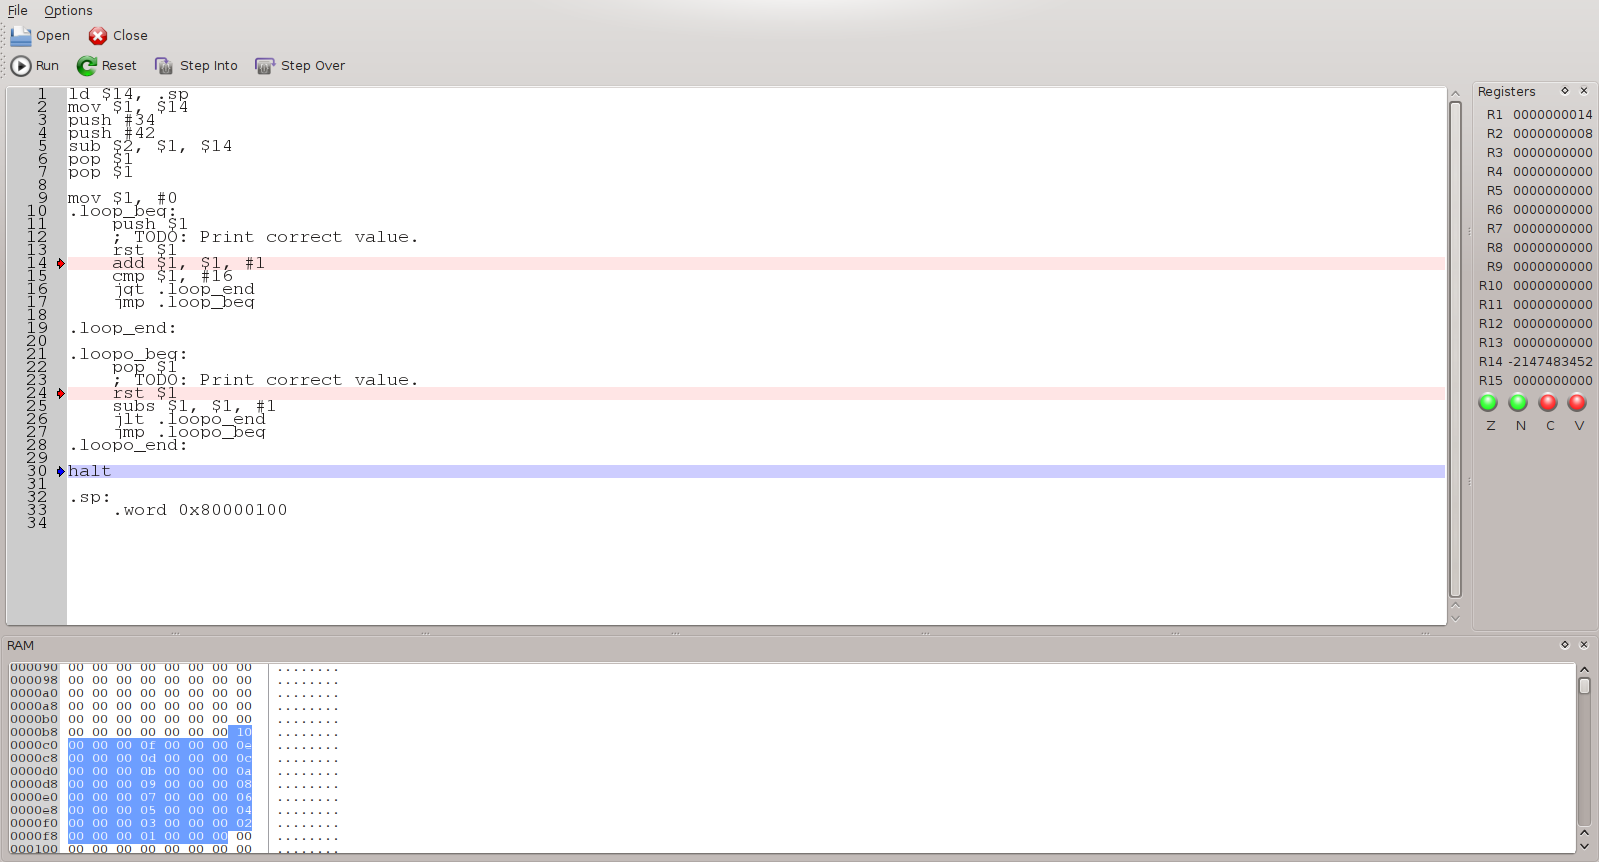
\includegraphics[width=\textwidth]{images/debugger.png}
\captionof{figure}{\label{SW:debugger}Screenshot des Debuggers}
\end{figure}
Wie in \autoref{SW:debugger} zu sehen ist, sind alle wichtigen Informationen der CPU zu sehen -- Registerinhalte, Programmcounter, Statusregister und Ram-Inhalt.
Auch die Manipulation von Werten ist möglich, so z.B. des Raminhalts, der Register und er Statusflags. Man kann desweiteren Breakpoints setzen und Programmteile überspringen oder genauer inspizieren.\\
Die Oberfläche wurde mit dem Qt-Designer kreiert, das Programm selbst in wie der Rest in Python geschrieben.
